\cotefile{154}
\scanpage{62}
% archive sheet number: 61
% printed form
{\ttfamily\small\raggedright
\$HASP373 STARTED - INIT 2 - CLASS 1 - SYS E333\\
IEF236I ALLOC. FOR CRAY2\\
IEF142I CRAY2 - STEP WAS EXECUTED - COND CODE 0000\\
IEF373I STEP / \hspace{1em} / START 82229.0906\\
IEF374I STEP / \hspace{1em} / STOP 82229.0906 CPU 0MIN 00.01SEC SRB 0MIN 00.00SEC VIRT 8K SYS 200K\\
IEF375I JOB /CRAY2 \hspace{1em} / START 82229.0906\\
IEF376I JOB /CRAY2 \hspace{1em} / STOP 82229.0906 CPU 0MIN 00.01SEC SRB 0MIN 00.00SEC\par}

\diagram{\handwritten{\begin{tikzcd}[ampersand replacement=\&,column sep=large]
 F=F_D \arrow[r] \& F_{D'}=F'
\end{tikzcd}}}

\figure{\handwritten{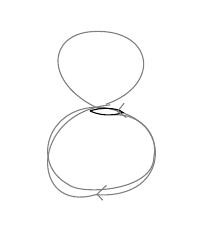
\begin{tikzpicture}[scale=.7]
\draw[thin,gray] (0,.04) .. controls (-1,.5) and (-.94,1.4) .. (-.1,1.44)
 .. controls (.98,1.5) and (1.16,.48) .. (.13,.12);
\draw[gray] (.1,.06) .. controls (-.9,.16) and (-1.27,-.94) .. (-.56,-1.33)
 .. controls (-.35,-1.53) and (.99,-1.47) .. (1,-.84)
 .. controls (1.1,-.32) and (.63,-.04) .. (.1,.06);
\draw[thin,gray] (.21,.11) .. controls (-1.28,-.03) and (-1.24,-1.87) .. (-.06,-1.52)
 .. controls (1.4,-1.62) and (1.26,-.03) .. (.28,-.07);
\draw (-.16,0) .. controls (.04,.07) and (.34,.06) .. (.44,-.03)
 .. controls (.24,-.1) and (0,-.08) .. (-.16,0);
\draw[thin,gray] (.46,.14)--(.34,-.01)--(.5,-.12);
\draw[thin,gray] (.14,-1.35)--(-.03,-1.51)--(.07,-1.62);
\end{tikzpicture}}}

\diagram{\handwritten{\begin{tikzcd}[ampersand replacement=\&,column sep=7em,row sep=2.4em]
\omega(F_D) \arrow[r,"{\alpha\ \text{transport parallèle}}","{\text{cond. via les}\ \mathrm{Pol}(D)}"'] \arrow[d,phantom,"\rotatebox{90}{$\simeq$}" description] \& \omega(F_{D'}) \arrow[d,phantom,"\rotatebox{90}{$\simeq$}" description]\\
\omega(\deleted{\unsure{\partial}}F\deleted{\unsure{,}}) \arrow[r,"{\beta\ \text{transport de}}","{\text{l'orientation sur }\unsure{\mathscr X|X|\mathcal X}}"'] \arrow[d,phantom,"\rotatebox{90}{$\simeq$}" description] \& \omega(F') \arrow[d,phantom,"\rotatebox{90}{$\simeq$}" description]\\
\omega(D) \arrow[r,"{\alpha'\ \text{transport parallèle}}"] \& \omega(D')
\end{tikzcd}}}

\figure{\handwritten{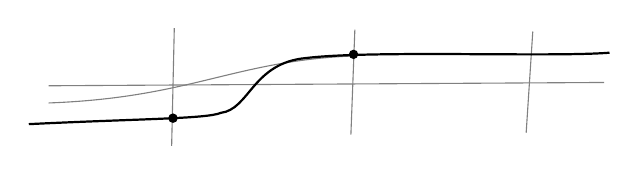
\begin{tikzpicture}[x=.84cm,y=.84cm]
\draw[thin,gray] (0,.48)--(8.4,.53);
\draw[thin,gray] (0,.22) .. controls (2.15,.3) and (2.78,.85) .. (4.58,.93);
\draw[thin,gray] (1.86,-.43)--(1.90,1.35) (4.57,-.26)--(4.63,1.33) (7.22,-.23)--(7.32,1.3);
\draw[thick] (-.3,-.1) .. controls (1.34,-.02) and (2.4,-.02) .. (2.6,.07)
 .. controls (3.04,.12) and (3.08,.83) .. (3.9,.9)
 .. controls (4.9,1.02) and (7.6,.91) .. (8.48,.98);
\fill (1.88,-.01) circle (.072) (4.61,.955) circle (.071);
\end{tikzpicture}}}

\handwritten{$\alpha=\alpha'$, \quad $\beta=\alpha,\alpha'$ ssi nb d'opérations \inserted{$N$} est pair}

\handwritten{\uline{ex} \quad $F=F_{D'}$, \quad $\alpha=\alpha'=-1$ \quad alors $\beta=-1$ ssi \deleted{\unsure{nb|tel}} $N$ pair}

\handwritten{donc}
